\documentclass[10pt]{article}
\usepackage[utf8]{inputenc}
\usepackage[T1]{fontenc}
\usepackage{amsmath}
\usepackage{amsfonts}
\usepackage{amssymb}
\usepackage[version=4]{mhchem}
\usepackage{stmaryrd}
\usepackage{graphicx}
\usepackage[export]{adjustbox}
\graphicspath{ {./images/} }

\title{Università di Catania 
 Corso di Laurea in Fisica 
 Compito scritto di Fisica Generale I 
 M.G. Grimaldi - A. Insolia }

\author{}
\date{}


\begin{document}
\maketitle
Per la prova in itinere ( 2 ore) svolgere i problemi: \(3,4,5\)

Catania, 7 Settembre 2022

Per la prova completa (3 ore) svolgere i problemi: \(1,2,3,4\)

\section{Problema n.1}
Un corpo viene lanciato verso l'alto. Raggiunto il punto di quota massima \(h\) all'istante \(t=0\), esso si divide in tre parti di massa uguale. Uno dei tre frammenti, di velocità iniziale \(\mathrm{v}_{1}\) diretta verticalmente (vedi figura) raggiunge il suolo all'istante \(t_{1}=4 \mathrm{~s}\), gli altri due atterrano insieme all'istante \(t_{2}=5 \mathrm{~s}\). Determinare:

a) la quota massima \(h\) raggiunta dal corpo prima dell'esplosione;

b) le componenti lungo y delle velocità dei tre frammenti al momento dell'esplosione.

\begin{center}
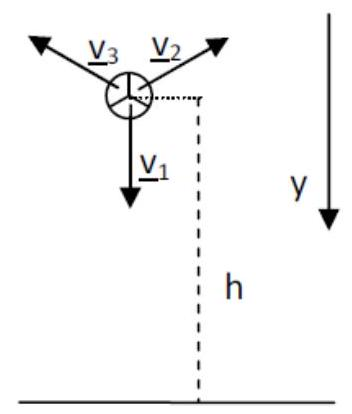
\includegraphics[max width=\textwidth]{2023_05_14_f312833f6ad620ab7ea5g-1(1)}
\end{center}

\section{Problema n.2}
Gli assi di due cilindri pieni, aventi lo stesso raggio \(\mathrm{R}=20 \mathrm{~cm}\) e masse \(\mathrm{m}_{1}=20 \mathrm{~kg} \mathrm{e} \mathrm{m}_{2}=30 \mathrm{~kg}\), sono collegati da una sbarra rigida di massa trascurabile (vedi figura). Ciascun cilindro può ruotare liberamente attorno al proprio asse. All' asse del cilindro 1 è applicato un momento di modulo \(\mathrm{M}\) ed il pavimento su cui sono appoggiati i cilindri presenta un coefficiente di attrito statico \(\mu_{s}=0.50\). Determinare:

a) la massima accelerazione (dei centri di massa), \(a_{\max }\) con cui i due cilindri avanzano di puro rotolamento;

b) il valore di \(M, M_{\max }\), che deve agire sul cilindro 1 nella situazione del punto a).

[Si noti che, a causa dell'asta che connette i due cilindri, questi hanno la stessa accelerazione angolare]

\begin{center}
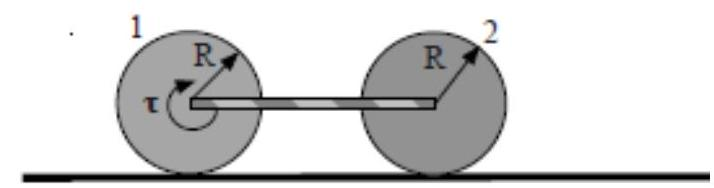
\includegraphics[max width=\textwidth]{2023_05_14_f312833f6ad620ab7ea5g-1}
\end{center}

\section{Problema n.3}
Un corpo di volume \(V\) e avente densità \(\rho_{c}=0.800 \mathrm{~g} / \mathrm{cm}^{3}\), partendo dalla quiete e dopo aver percorso in caduta libera in aria una distanza \(h_{A}=1.00 \mathrm{~m}\), entra in una vasca contenente acqua. Trascurando la viscosità, calcolare la massima profondità \(h_{B}\) (rispetto alla superficie libera dell'acqua) raggiunta dal corpo.

\section{Problema n.4}
Una mole di gas ideale monoatomico, partendo dallo stato A caratterizzato da \(V_{A}=8 \mathrm{dm}^{3}\) e \(T_{2}=500\) \(\mathrm{K}\), compie un ciclo termodinamico reversibile costituito, nell'ordine, da: una trasformazione isoterma fino allo stato \(B\) con \(\mathrm{V}_{\mathrm{B}}=2 \mathrm{~V}_{\mathrm{A}}\), una espansione adiabatica fino allo stato \(C\) caratterizzato da \(T_{0}=260 \mathrm{~K}\), una trasformazione isoterma fino allo stato \(D\) con \(\mathrm{V}_{\mathrm{D}}=6 \mathrm{~V}_{\mathrm{B}}\), una compressione adiabatica fino allo stato \(E\) con \(T_{1}=360 \mathrm{~K}\), una compressione isoterma fino allo stato \(F\) e quindi una compressione adiabatica che riporta il sistema alla condizione iniziale \(A\).

a) Scelto un valore arbitrario di riferimento per l'entropia del sistema in A, disegnare il ciclo termodinamico su un diagramma S-T (con S entropia del sistema).

b) Calcolare il calore totale scambiato nel ciclo.

c) Determinare il rendimento del ciclo.

\section{Problema n.5}
Un pezzetto di ghiaccio di massa \(m\) e alla temperatura di \(\mathrm{T}_{1}=250 \mathrm{~K}\) viene immerso in \(m_{2}=60 \mathrm{~g}\) di acqua a temperatura di \(\mathrm{T}_{2}=330 \mathrm{~K}\). Se il sistema e contenuto in un recipiente a pareti adiabatiche:

a) si determini per quali valori della massa \(m\) il pezzetto di ghiaccio fonde completamente;

b) calcolare la temperatura di equilibrio del sistema se la massa del cubetto di ghiaccio vale \(\quad\) g. II calore specifico del ghiaccio vale \(\mathrm{c}_{\mathrm{g}}=2051 \mathrm{~J} / \mathrm{KgK}\), il calore specifico dell'acqua vale \(\mathrm{c}_{\mathrm{a}}=4186.8 \mathrm{~J} / \mathrm{KgK}\) ed il calore latente di fusione del ghiaccio e pari a \(\lambda_{f}=3.3 \times 10^{5} \mathrm{~J} / \mathrm{Kg}\).


\end{document}